\titre{Question 1} \\Non car intégrité = vérifier que la donnée est restée identique -> inutile de savoir qui s'en sert.
	\begin{itemize}
		\item A t'on besoin d'assurer l'intégrité pour pouvoir authentifier ? Non
		\item A t'on besoin d'authentification pour assurer l'intégrité ? Non
	\end{itemize}

\titre{Question 2}
	\begin{itemize}
		\item confidentialité Non
		\item authentification Oui car pour attribuer une action à quelqu'un il faut l'avoir authentifié
		\item intégrité Oui car il faut que les preuves soient intègres
		\item contrôle d'accès Non
	\end{itemize}

\titre{Question 3} \\
	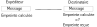
\includegraphics[width=200px]{Images/01_integrite.pdf}\\
	\includegraphics[width=200px]{Images/02_chiffrement1.pdf}\\
	Autre méthode de confidentialité : authentification + contrôle d'accès\\
	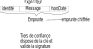
\includegraphics[width=200px]{Images/03_nonRepudiation.pdf}\\

\titre{Question 4} \\Une contrôleur de domaine est un serveur chargé de l'authentification. Domaine logique \\
	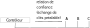
\includegraphics[width=200px]{Images/04_controle.pdf}\\

\titre{Question 5} Domaine physique

\titre{Question 6}
	\begin{itemize}
		\item Casiers judiciaires
		\item Dossiers médicaux
		\item Relevés bancaires
		\item Enquêtes de police
		\item Enquêtes fiscales
		\item Documents industriels confidentiels
		\item Délibérations du gouvernement
	\end{itemize}
	Les personnes concernées ont toujours le droit d'accéder à leurs informations personnelles.

\titre{Question 7}\\Commission Nationale Informatique et Liberté. La CNIL est une institution indépendante qui a pour rôle de faire respecter la loi informatique et libertés.

\titre{Question 8}\\La "politique de sécurité" est un document qui détermine les objets à sécuriser, identifie les menaces à prendre en compte, définit le périmètre de sécurité et spécifie l'ensemble des lois, règlements et pratiques à respecter pour assurer la sécurité.

\titre{Question 9}\\On écrit le plan, puis on le teste (on provoque une panne et on essaye de faire une reprise d'activité). C'est cette phase qui est la plus dure à réaliser.
	\begin{itemize}
		\item Vérifier l'intégrité des données
		\item Réparer les données corrompues
		\item Récupérer les données à partir d'archives
	\end{itemize}

\titre{Question 10}\\La sécurité est l'affaire de tous. L'élément humain est le plus problématique car :
	\begin{itemize}
		\item Pas conscient des enjeux
		\item Sécurité = contraignant (ex : interdiction de clé USB, mdp complexes, sites web inaccessibles etc)
	\end{itemize}

\titre{Question 11}
	\begin{itemize}
		\item Perte de l'appareil $\impl$ perte des données stockées $\impl$ perte de confidentialité
		\item Utilisation de services cloud pour stocker des données sensibles
		\item Présence de virus sur la machine
		\item etc
	\end{itemize}
